\documentclass[12pt]{article}

\usepackage{geometry}
\usepackage[utf8]{inputenc}
\usepackage[T2A]{fontenc}
\usepackage[russian]{babel}
\usepackage{graphicx}
\usepackage{caption}
\usepackage{amssymb, gensymb, amsmath}
\usepackage{mathrsfs}
\usepackage{array, colortbl}
\usepackage{multicol}

\title{{\bf Лабораторная работа 1.\, 3. \\ Изучение рассеяния медленных электронов на атомах (эффект Рамзауэра)}}
\author{Лось Денис (группа 618)}
\date{13 сентября 2018}

\begin{document}

\maketitle

\paragraph{Цель работы: } исследовать энергетическую зависимость вероятности рассеяния электронов атомами ксенона, определить энергии электронов, при которых наблюдается "просветление" ксенона и оценить размер его внешней электронной оболочки.

\section*{Теоритическое введение}
\par
	Сделаем учет волной природы электронов и дадим объяснение эффекту Рамзауэра. Схема эксперимента показана на рис.1.
\begin{figure}[h!]
	\centering
	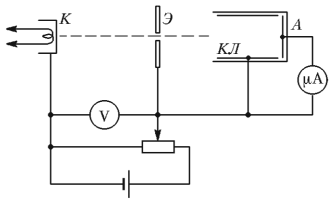
\includegraphics[width = 8cm, height = 5cm]{image3.png}
	\caption{Схема установки для измерения сечения рассеяния электронов в газах}
\end{figure}
\par
	Пучок электронов, вылетая из накаленного катода К, проходит ускоряющую разность потенциалов $V$, приложенную между катодом и электродом Э,и приобретаем тем самым энергию $E = \frac{m v^2}{2} = e V$. При прохождении через газ часть электронов рассеивается на атомах, уходит в сторону и собирается коллектором, а прошедшие без рассеяния электроны попадают на анод А и создают анодный ток $I$. Ток $I$ пропорционален числу прошедших электронов, и поэтому непосредственно характеризует проницаемость газа для электронного пучка в зависимости от его скорости (ускоряющего напряжения). Согласно классическим воззрениям с ростом напряжения $V$, как оказалось выше, сечение рассеяния уменьшается, и ток должен монотонно возрастать.
\par
	С точки зрения квантовой теории картина рассеяния выглядит иначе. Внутри атома потенциальная энергия налетающего электрона $U$ отлична от нуля, скорость электрона изменяется, становясь равной $v'$ в соотвествии с законом сохранения энергии
\[
	E = \frac{m v^2}{2} = \frac{m v'^2}{2} + U,
\]
а значит, изменяется и длина его волны де Бройля. Таким образом, по отношению к электронной волне атом ведет себя как преломляющая среда с относительным показателем преломления 
\begin{equation}
	n = \frac{\lambda}{\lambda'} = \sqrt{1 - \frac{U}{E}}.
\end{equation}
\par
	Для упрощения задачи будем использовать модель прямоугольной потенциальной ямы. В результате рассматриваем задачу о прохождении частицы с энергией $E$ над потенциальной ямой шириной $l$ и глубиной $U_0$.
\par
	Уравнение Шредингера в данном случае имеет вид
\[
	\psi'' + k^2 \psi = 0,
\]
где $k^2 = k_1^2 = 2 m E / h^2$ --- в областях 1 и 3, $k^2 = k_2^2 = 2 m (E + U_0) / h^2$ --- в областях 2.
\begin{figure}[h!]
	\centering
	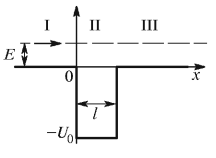
\includegraphics[width = 8cm, height = 5cm]{image4.png}
	\caption{Схематическое изображение прямоугольной ямы, над которой пролетает частица с энергией $E$}
\end{figure}
\par
	Коэффициент прохождения равен отношению квадратов амплитуд прошедшей и падающей волн и определяется выражением
\begin{equation}
	D = \frac{16 k_1^2 k_2^2}{16 k_1^2 k_2^2 + 4 (k_1^2 - k_2^2)^2 sin^2(k2 l)},
\end{equation}
\par
	Можем заметить, что коэффиент прохождения частицы над ямой имеет, в зависимости от её энергии, ряд чередующих максимумов и минимумов. В частности, если $k_2 l = \pi$, то $\sin k_2 l = 0$ и коэффициент прохождения равен единице, т.е. отражённая волна отсутствует, и электрон беспрепятственно проходит через атом, что явлется квантовым аналогом просветления оптики.
\par
	Следовательно, коэффициент прохождения электронов максимален при условии
\begin{equation}
	k_2 l = \sqrt{\frac{2 m (E + U_0)}{h^2} l} = n \pi, \quad n = 1, 2, \dots
\end{equation}
\par
	Данное условие мы также можем получить, если будем рассматривать интерференцию электронных волн де Бройля в атоме. Движущемуся электрону соответствует волна де Бройля, длина которой определяется соотношением $\lambda = h / mv$. Если кинетическая энергия электрона невелика, то $E = mv^2 / 2$ и $\lambda = h / \sqrt{2mE}$. При движении электрона через атом длина волны де Бройля становится меньше и равна $\lambda' = h / \sqrt{2m (E + U_0}$, где $U_0$ --- глубина атомного потенциала. При этом, волна де Бройля отражается от поверхности атома и происходит интерференция прошедшей через атом волны и отраженной от передней и задней границы атома (эти волны когерентны).
\par
	Прошедшая волна усилится отраженной волной, если геометрическая разность хода между ними $\Delta = 2 l = \lambda'$, что соответствует условию первого интерференционного максимума, т.е. при условии
\[
	2 l = \frac{h}{\sqrt{2m (E_1 + U_0)}}
\] 
\par
	С другой стороны, прошедшая волна ослабится, если $\Delta = 2l = (3/2)\lambda'$ (условие первого интерференционного минимума), т.е. при условии
\[
	2 l = \frac{3}{2} \frac{h}{\sqrt{2m (E_2 + U_0)}}
\]
\par
	Решив совместно эти два уравнения и исключив $U_0$, можем найти эффективный размер атома
\begin{equation}
	 l = \frac{h \sqrt{5}}{\sqrt{32 m (E_2 - E_1)}}
\end{equation}
\par
	Так как энергии $E_1$ и $E_2$ соответствуют энергиям электронов, прошедших разность потенциалов $V_1$ и $V_2$, т.е. $E_1 = e V_1$ и $E_2 = e V_2$, то по измеренным величинам $E_1$ и $E_2$ можем рассчитать эффективную глубину потенциальной ямы атома:
\[
	U_0 = \frac{4}{5} E_2 - \frac{9}{5} E_1.
\]
\section*{Экспериментальная установка}
\par
	В работе для изучения эффекта Рамзауэра используется тиратрон, заполненный инертным газом. Схематическое изображение тиратрона и его конструкция приведены на рис.\ref{TIR}.
\begin{figure}[h!]
	\centering
	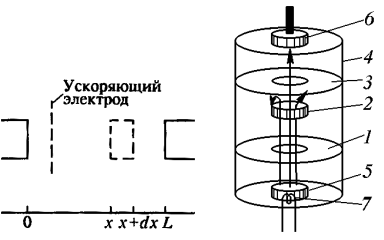
\includegraphics[width = 8cm, height=4cm]{image1.png}
	\caption{Схематическое изображение тиратрона и его конструкция}
	\label{TIR}
\end{figure}
\par
	Электроны, эмитируемые катодом тиратрона,ускоряются напряжением $V$, приложенным между катодом и ближайшей к нему сеткой. Затем электроны рассиваются на атомах инертного газа (ксенона). Все сетки 1, 2, 3 соединены между собой и имеют одинаковых потенциал, примерно равный потенциалу анода 6. Поэтому между первой сеткой и анодом практически нет поля. Рассеянные электроны отклоняются в сторону и уходят на сетку, а оставшееся часть электронов достигает анода и создаёт анодный ток $I_\text{а}$. Таким образом, поток электронов $N(x)$ на расстоянии $x$ от ускоряющей сетки (т.е число электронов, проходящих через поперечное сечение лампы в точке $x$ в единицу времени) уменьшается с ростом $x$ от начального значения $N_0$ у катода (в точке $x = 0$) до некоторого значения $N_\text{а}$ у анода (в точке $x = L$).
\par
	Раccмотрим теперь, какова должна быть реальная вольтамперная характеристика тиратрона. Выделим в газе на расстоянии $x$ от катода тонкий слой с площадью поперечного сечения $S$  и толщиной $dx$. Этот слой содержит $dv = n_\text{а} S dx$ атомов газа ($n_\text{а}$ --- концентрация атомов газа в лампе). Суммарное рассеивающая поверхность этих атомов (суммарное эффективное сечение рассеяния) $\Delta = v \Delta_\text{а}$, где $\Delta_\text{а}$ --- площадь поперечного сечения атома. Обозначим через $dN$ убыль потока электронов в результате прохождения слоя $dx$, тогда $dN/N(x)$ есть доля рассеянных электронов, или вероятность рассеяния в слое. Для рассеяния электрона в слое необходимо выполнение друх независимых событий --- вероятности для электрона в слое $dx$ встретить атома (она равна $\Delta/S$ --- доли площади поперечного сечения слоя, перекрываемого атомами) и вероятности рассеяния на атоме $\omega(V)$:
\begin{equation}
	- \frac{dN}{N(x)} = \frac{\Delta}{S} \omega(V) = n_\text{а} \Delta_\text{а} \omega(V) dx.
\end{equation}
\par
	Интегрируя это соотношение от $0$ до $L$ и заменяя поток электронов на ток $I = N e$, получаем уравнение ВАХ:
\begin{equation}
	I_\text{а} = I_\text{0} e^{-C \omega(V)}, \quad C = L n_\text{а} \Delta_\text{а}, \label{13}
\end{equation}
где $I_\text{0} = e N_\text{0}$ --- ток катода, $I_\text{а} = e N_\text{а}$ --- анодный ток.
\par
	Согласно классическим представлениям сечение рассеяния электрона на атоме должно падать монотонно с ростом $V$ (обратно пропорционально скорости электрона, т.е. обратно пропорционально квадратному корню из его энергии), а значит, ВАХ будет монотонно возрастающей функцией, как показано на рисунке а). По квантовым соображениям вероятность рассеяния электронов и соответствующая ВАХ должны иметь вид, показанный на рисунке б).
\newpage
\begin{figure}[h!]
	\centering
	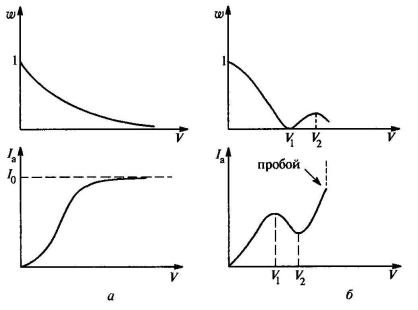
\includegraphics[width = 12cm, height = 8cm]{image2.png}
	\caption{Качественный вид вероятности рассеяния электрона атомом инертного газа и ВАХ тиратрона при классическом (а) и квантовом (б) рассмотрении}
\end{figure}
\par
	Согласно формуле \ref{13} по измеренной ВАХ тиратрона можно определить зависимость вероятности рассеяния электрона от его энергии из соотношения
\begin{equation}
	\omega(V) = - \frac{1}{C} \ln\frac{I_\text{а}(V)}{I_0}.
\end{equation}
\par
	Блок схема используемой экспериментальной установки выглядит как
\begin{figure}[h!]
	\centering
	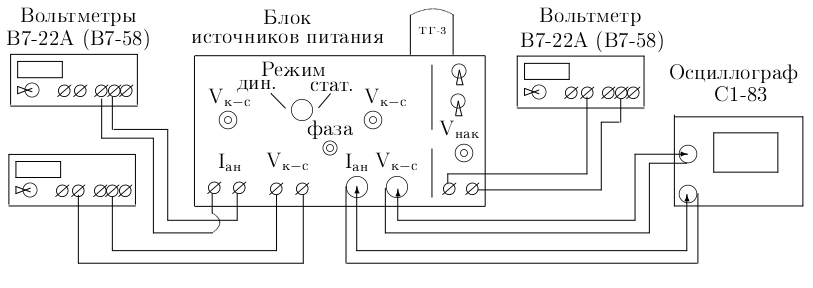
\includegraphics[width = 12cm, height = 5cm]{image6.png}
	\caption{Блок схема экспериментальной установки}
\end{figure}

\section*{Ход работы и результаты измерений}
\par
	Мы хотим получить изображения ВАХ эффекта на осциллографе, измерить расстояние между характерными точками в вольтах, снять ВАХ в статическом режиме; по результатам измерений рассчитать размер электронной оболочки атома, оценить глубину потенциальной ямы и потенциал ионизацию газа, заполняющего лампу.

\subsection*{Вольт-амперная характеристика тиратрона $I_\text{а} = f(U_\text{c})$ в динамическом режиме}

\par
	Установим напряжение накала равным $V_\text{накала} \approx 3	$ В и $V_\text{накала} \approx 2.8$ В. При максимальном ускоряющем напряжении отражённое относительно вертикальной оси изображение вида ВАX тиратрона:
\begin{figure}[h!]
	\centering
	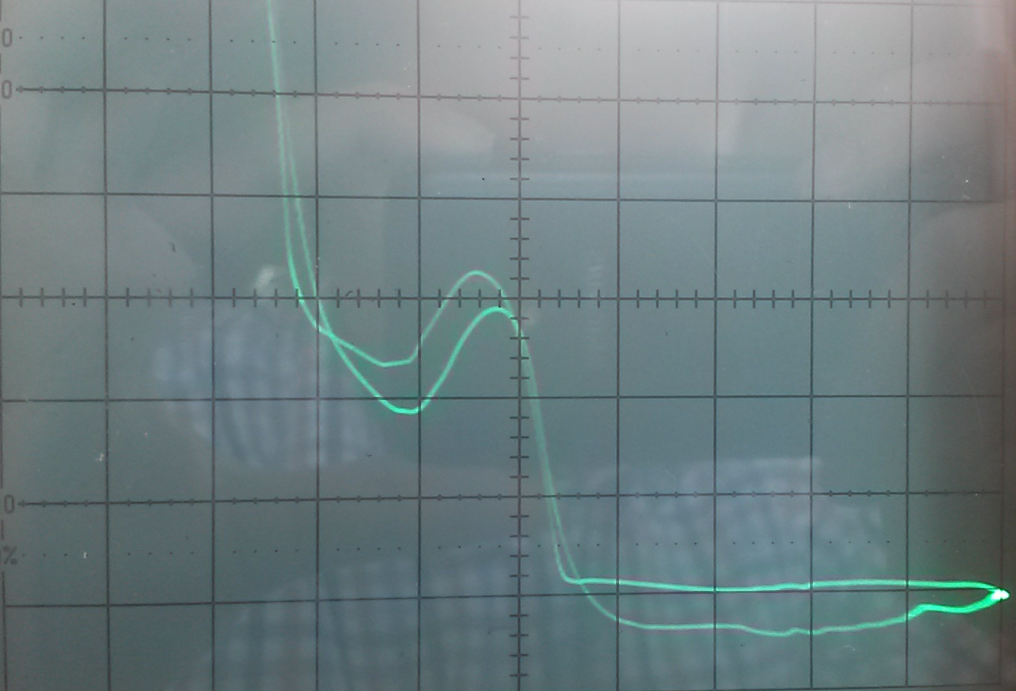
\includegraphics[width = 10cm, height = 6cm]{imageplot1.png}
	\caption{Осциллограмма при $V_\text{накала} = 3$ B}
\end{figure}
\par
	Измерим напряжения между катодом и сеткой, соотвествующие первому максимуму и минимуму на осциллограмме. Оценим также напряжение пробоя, соответствующее резкому скачку тока в конце кривой. Чувствительность канала X равна $5 \text{В}/\text{дел}$. Ноль по оси X находится в точке $U_x = 4$ В (4 доли деления). Однако мы видим характерный пологий участок на обоих графиках и графиков со статического режима.
\newpage
\begin{table}[h!]
	\centering
	\begin{tabular}{|c|c|}
	\hline
		$U_\text{max1}$, В  & 3\\
	\hline
		$U_\text{min1}$, В & 8\\
	\hline
		$U_\text{пробоя}$, В & 12\\
	\hline
	\end{tabular}
\end{table}
\begin{figure}[h!]
	\centering
	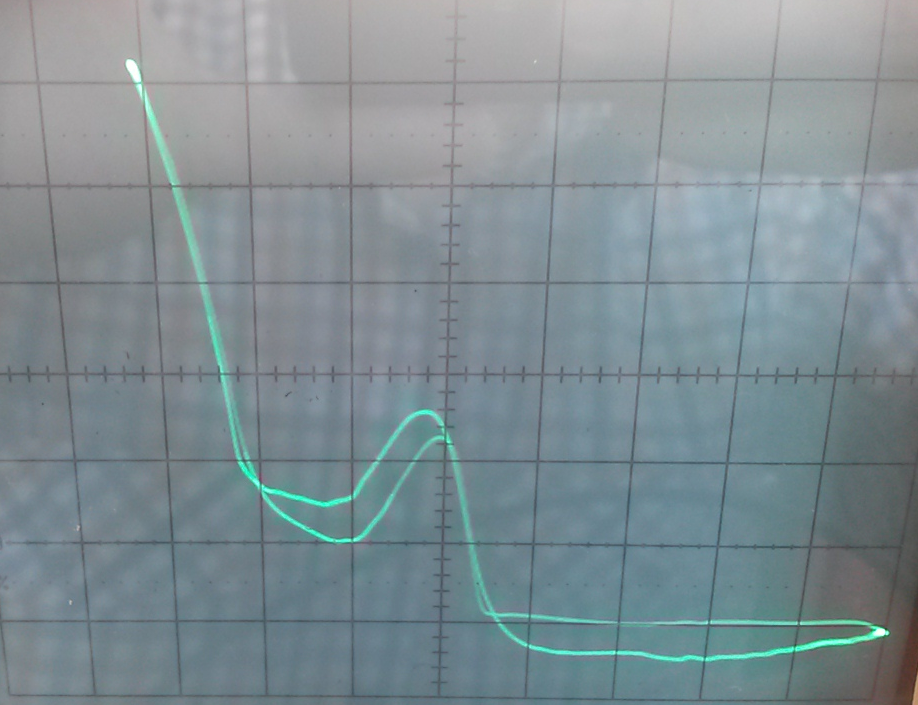
\includegraphics[width = 10cm, height = 6cm]{imageplot2.png}
	\caption{Осциллограмма при $V_\text{накала} = 2.8$ В}
\end{figure}
\par
	Так как напряжение пробоя практически совпадает с потенциалом ионизации, то ионизационный потенциал газа равен 12 эВ, что подтвержает информацию от том, что используется в установке газ ксенон с ионизационным потенциалом 12.1 эВ.
\par
	Оценим глубину потенциальной ямы $U_0 = e * (4/5 * U_\text{max1} - 1.8 * U_\text{min1}) =  1 $ эВ.
\par
	Оценим размер электронной оболочки атома газа, используя $E_2 = e U_\text{min1}$, и $E_1 = e U_\text{max1}$
\[
	l = \frac{h \sqrt{5}}{\sqrt{32m (E_2 - E_1)}}
\]
\par
	В результате получим $l = 0.3$ нм, что в принципе достаточно сильно отличается от табличного значения, так как согласно табличным данным $l = 2a = 0.216$ нм.  

\subsection*{Вольт-амперная характеристика $I_\text{а} = f(U_\text{с}$) в статическом режиме}

	В данном случае ток анода $I_\text{а}$ будет определяться по показанию вольтметра, делённому на сопротивление 100 кОм, включённое в цепь анода. Проведём измерения ВАХ тиратрона также для 2-х значений напряжения накала(тех же что и в динамическом режиме).
\par
	Проведём измерения для напряжения накала $V_\text{накала} = 3$ В и $V_\text{накала} = 2.8$ В и построим графики ВАХ.
\begin{figure}[h!]
	\centering
	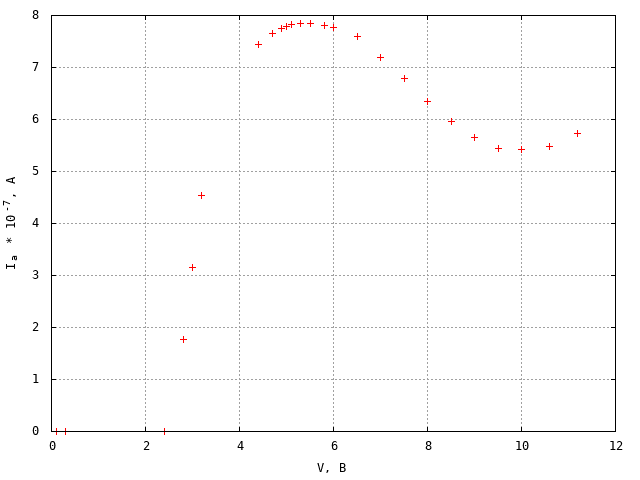
\includegraphics[width = 8cm, height= 4.5cm]{plot1.png}
	\caption{ВАХ при $V_\text{накала} = 3$ В}
\end{figure}
\begin{figure}[h!]
	\centering
	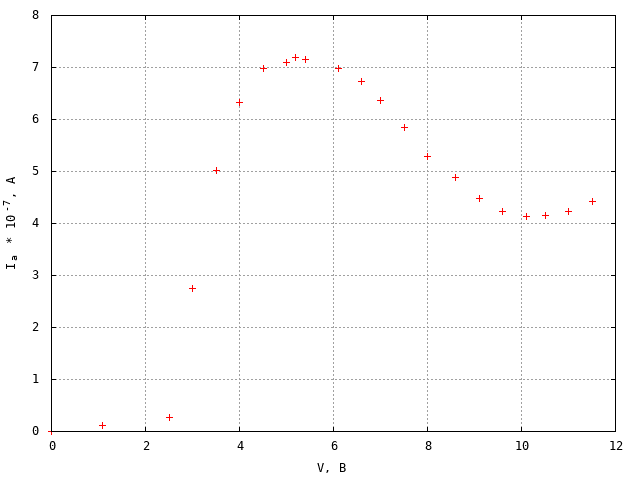
\includegraphics[width = 8cm, height= 4.5cm]{plot2.png}
	\caption{ВАХ при $V_\text{накала} = 2.8$ В}
\end{figure}
\begin{table}[h!]
\parbox{.5\linewidth}{
\centering
\begin{tabular}{|c|c|}
	\hline
		$U$, В & $I_a * 10^{-7}$, А \\
	\hline
		0.1	& 0 \\
	\hline
0.3	&0.01 \\
\hline
2.4	&0.01 \\
\hline
2.8	&1.76 \\
\hline
3.0	&3.16 \\
\hline
3.2	&4.53 \\
\hline
4.4	&7.45 \\
\hline
4.7	&7.66 \\
\hline
4.9	&7.74 \\
\hline
5.0	&7.78 \\
\hline
5.0	&7.79 \\
\hline
5.1	&7.83 \\
\hline
5.5	&7.85 \\
\hline
5.3	&7.84 \\
\hline
5.8	&7.82 \\
\hline
6.0	&7.77 \\
\hline
6.5	&7.60 \\
\hline
7.0	&7.20 \\
\hline
7.5	&6.78 \\
\hline
8.0	&6.35 \\
\hline
8.5	&5.96 \\
\hline
9.0	&5.65 \\
\hline
9.5	&5.44 \\
\hline
10.0&	5.42 \\
\hline
10.6&	5.48 \\
\hline
11.2&	5.72 \\
	\hline
	\end{tabular}
	\caption{Измерения для $V_\text{накала} = 3$ В}
}
\hfill
\parbox{.5\linewidth}{
\centering
\begin{tabular}{|c|c|}
	\hline
		$U$, В & $I_a * 10^{-7}$, А \\
\hline
	1.1&	0.11 \\
\hline
2.5	&0.27 \\
\hline
3.0	&2.75 \\
\hline
3.5	&5.02 \\
\hline
4.0&	6.32 \\
\hline
5.0	&7.10 \\
\hline
6.1	&6.98 \\
\hline
5.4	&7.16 \\
\hline
4.5	&6.98 \\
\hline
5.2	&7.20 \\
\hline
6.6	&6.74 \\
\hline
7.0&	6.36 \\
\hline
7.5	&5.84 \\
\hline
8.0	&5.28 \\
\hline
8.6&	4.88 \\
\hline
9.1&	4.49 \\
\hline
9.6	&4.24 \\
\hline
10.1&	4.14 \\
\hline
10.5&	4.15 \\
\hline
11.0&	4.24 \\
\hline
11.5&	4.43 \\
\hline
\end{tabular}
\caption{Измерения для $V_\text{накала} = 2.8$ В}
}
\end{table}
\par

\end{document}